\documentclass[border=8pt]{standalone}
\usepackage{amsmath,amssymb}
\usepackage{tikz}
\usetikzlibrary{positioning, arrows.meta, calc}
\usepackage[T1]{fontenc}

\begin{document}
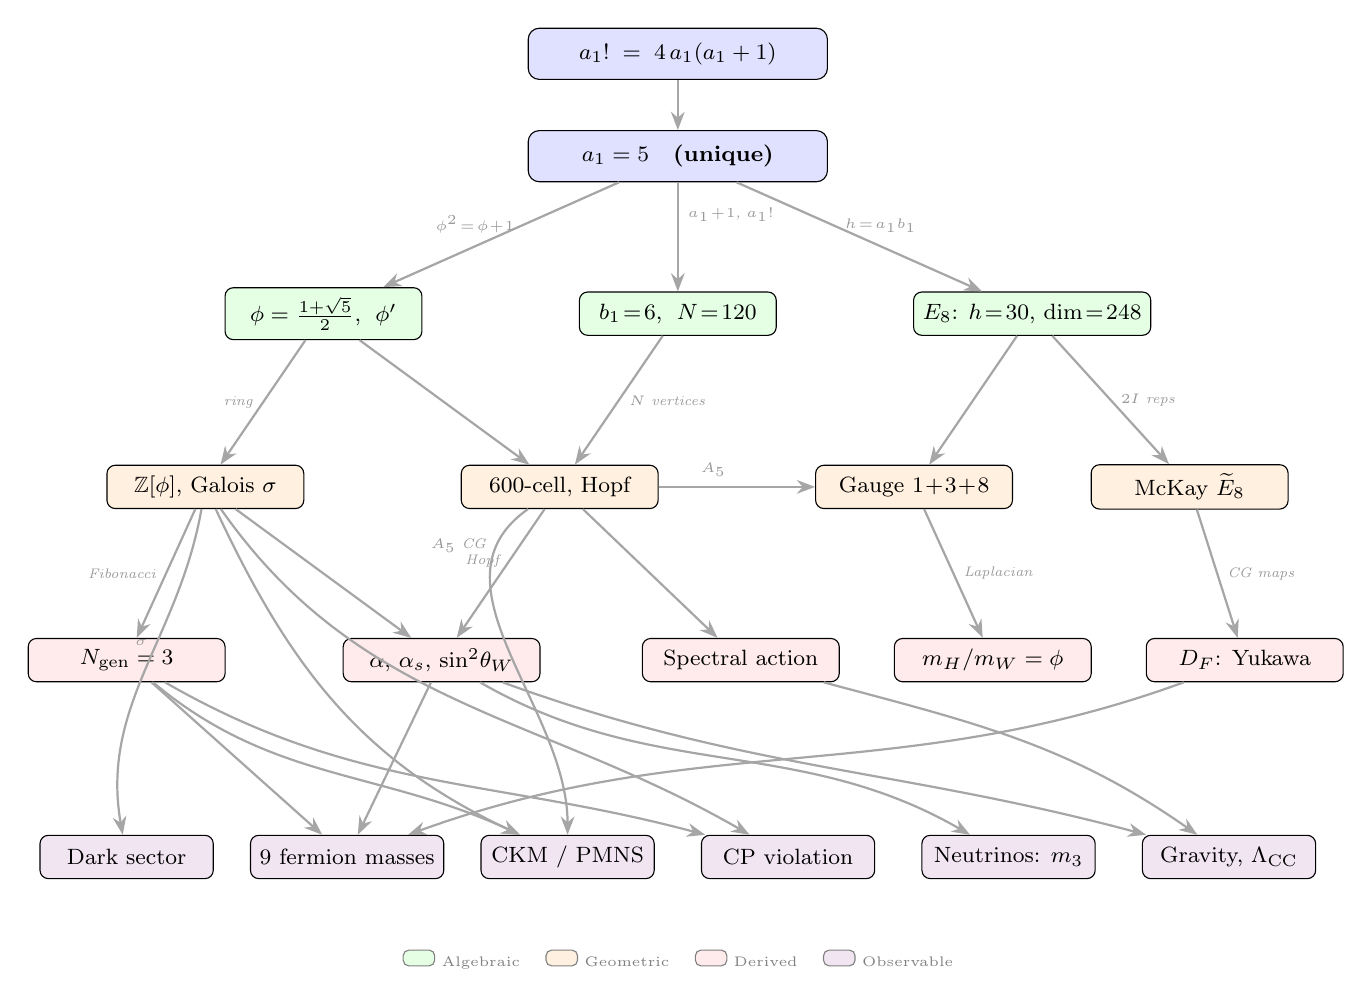
\begin{tikzpicture}[
  >=Stealth,
  every node/.style={font=\footnotesize},
  root/.style={draw, rounded corners=4pt, fill=blue!12, font=\footnotesize\bfseries,
               minimum width=3.8cm, minimum height=0.65cm, align=center},
  alg/.style={draw, rounded corners=3pt, fill=green!10,
              minimum width=2.5cm, minimum height=0.55cm, align=center},
  geo/.style={draw, rounded corners=3pt, fill=orange!12,
              minimum width=2.5cm, minimum height=0.55cm, align=center},
  phys/.style={draw, rounded corners=3pt, fill=red!8,
               minimum width=2.5cm, minimum height=0.55cm, align=center},
  obs/.style={draw, rounded corners=3pt, fill=violet!10,
              minimum width=2.2cm, minimum height=0.55cm, align=center},
  arr/.style={->, thick, gray!70},
  lbl/.style={font=\tiny\itshape, text=gray!80}
]

%--- Row 0: Root ---
\node[root] (dioph) at (0, 0) {$a_1!\;=\;4\,a_1(a_1+1)$};
\node[root] (a1) at (0, -1.3) {$a_1 = 5$ \;\;(unique)};
\draw[arr] (dioph) -- (a1);

%--- Row 1: Algebraic ---
\node[alg] (phi) at (-4.5, -3.3) {$\phi = \tfrac{1+\sqrt{5}}{2}$, \;$\phi'$};
\node[alg] (params) at (0, -3.3) {$b_1\!=\!6$, \;$N\!=\!120$};
\node[alg] (e8) at (4.5, -3.3) {$E_8$: $h\!=\!30$, $\dim\!=\!248$};

\draw[arr] (a1) -- node[lbl, left, pos=0.4]{$\phi^2\!=\!\phi\!+\!1$} (phi);
\draw[arr] (a1) -- node[lbl, right, pos=0.3]{$a_1\!+\!1$, $a_1!$} (params);
\draw[arr] (a1) -- node[lbl, right, pos=0.4]{$h\!=\!a_1 b_1$} (e8);

%--- Row 2: Geometric/Structural ---
\node[geo] (zphi) at (-6, -5.5) {$\mathbb{Z}[\phi]$, Galois $\sigma$};
\node[geo] (cell) at (-1.5, -5.5) {600-cell, Hopf};
\node[geo] (gauge) at (3, -5.5) {Gauge $1\!+\!3\!+\!8$};
\node[geo] (mckay) at (6.5, -5.5) {McKay $\widetilde{E}_8$};

\draw[arr] (phi) -- node[lbl, left]{ring} (zphi);
\draw[arr] (params) -- node[lbl, right]{$N$ vertices} (cell);
\draw[arr] (phi) -- (cell);
\draw[arr] (e8) -- (gauge);
\draw[arr] (e8) -- node[lbl, right]{$2I$ reps} (mckay);
\draw[arr] (cell) -- node[lbl, above, pos=0.35]{$A_5$} (gauge);

%--- Row 3: Derived physics ---
\node[phys] (ngen) at (-7, -7.7) {$N_{\text{gen}} = 3$};
\node[phys] (couplings) at (-3, -7.7) {$\alpha$, $\alpha_s$, $\sin^2\!\theta_W$};
\node[phys] (spectrum) at (0.8, -7.7) {Spectral action};
\node[phys] (higgs) at (4, -7.7) {$m_H/m_W = \phi$};
\node[phys] (df) at (7.2, -7.7) {$D_F$: Yukawa};

\draw[arr] (zphi) -- node[lbl, left]{Fibonacci} (ngen);
\draw[arr] (zphi) -- (couplings);
\draw[arr] (cell) -- node[lbl, left, pos=0.4]{Hopf} (couplings);
\draw[arr] (cell) -- (spectrum);
\draw[arr] (gauge) -- node[lbl, right]{Laplacian} (higgs);
\draw[arr] (mckay) -- node[lbl, right]{CG maps} (df);

%--- Row 4: Observables ---
\node[obs] (dark) at (-7, -10.2) {Dark sector};
\node[obs] (masses) at (-4.2, -10.2) {9 fermion masses};
\node[obs] (mixing) at (-1.4, -10.2) {CKM / PMNS};
\node[obs] (cp) at (1.4, -10.2) {CP violation};
\node[obs] (neutrinos) at (4.2, -10.2) {Neutrinos: $m_3$};
\node[obs] (gravcc) at (7, -10.2) {Gravity, $\Lambda_{\text{CC}}$};

%--- Arrows to observables ---

% Dark sector <- Galois conjugation
\draw[arr] (zphi) to[out=-100, in=100] node[lbl, left, pos=0.4]{$\sigma$} (dark);

% 9 fermion masses <- N_gen + couplings + D_F
\draw[arr] (ngen) -- (masses);
\draw[arr] (couplings) -- (masses);
\draw[arr] (df) to[out=200, in=20] (masses);

% CKM/PMNS <- A5 CG + Galois + N_gen
\draw[arr] (cell) to[out=-145, in=90] node[lbl, left, pos=0.15]{$A_5$ CG} (mixing);
\draw[arr] (zphi) to[out=-65, in=155] (mixing);
\draw[arr] (ngen) to[out=-40, in=155] (mixing);

% CP <- Galois Berry phase + N_gen
\draw[arr] (zphi) to[out=-55, in=150] (cp);
\draw[arr] (ngen) to[out=-30, in=165] (cp);

% Neutrinos <- couplings (seesaw)
\draw[arr] (couplings) to[out=-30, in=150] (neutrinos);

% Gravity + CC <- spectral + couplings
\draw[arr] (spectrum) to[out=-15, in=145] (gravcc);
\draw[arr] (couplings) to[out=-20, in=165] (gravcc);

%--- Legend ---
\node at (0, -11.5) [font=\tiny, text=gray] {
  \tikz\draw[fill=green!10,draw,rounded corners=2pt] (0,0) rectangle (0.4,0.2); Algebraic \quad
  \tikz\draw[fill=orange!12,draw,rounded corners=2pt] (0,0) rectangle (0.4,0.2); Geometric \quad
  \tikz\draw[fill=red!8,draw,rounded corners=2pt] (0,0) rectangle (0.4,0.2); Derived \quad
  \tikz\draw[fill=violet!10,draw,rounded corners=2pt] (0,0) rectangle (0.4,0.2); Observable
};

\end{tikzpicture}
\end{document}
